%!TEX program = xelatex
%windows、macOS用户都可用
\documentclass[UTF8, punct, oneside,fontset=none]{ctexbook}

\usepackage[windows]{template/latex/nsfc}
%macOS用户独享
%\documentclass[UTF8, punct, oneside]{ctexbook}
%\usepackage[macos]{nsfc}
%用来对比模版有无变化。对比时,请注释掉以下语句:
%\renewcommand{\input}[1]{\vspace{\baselineskip}}
%如果你个人文件和文件夹以⚠︎开头进行命名,可以省心更新模版。参见README.md
\usepackage[a4paper, left = 3.2cm, right = 3.2cm, top = 2.72cm, bottom = 2.54cm]{geometry}%页边距
\usepackage{times}
\usepackage{pifont}
\usepackage{setspace}
\usepackage{comment}
\usepackage{subfig}
\usepackage{tikz}

\pagestyle{empty} % 第二页以后页码空白
\graphicspath{{figures/}}   % 设置图片所存放的目录
\begin{document}
%\thispagestyle{empty}    % 首页页码空白

{\centering\zhkai\fontsize{16pt}{21pt}\selectfont
\setlength{\baselineskip}{21pt}%最后设置,防止被fontsize中的覆盖
\hspace{30pt}\textbf{报告正文}\par
\vspace{5.46pt}}%0.2(行距倍数)*21(行距)*1.3(word)

%\begin{comment}
{\zhkai\fontsize{14pt}{22pt}\selectfont
 \setlength{\baselineskip}{22pt}%最后设置,防止被fontsize中的覆盖
参照以下提纲撰写,要求内容翔实、清晰,层次分明,标题突出。
\textbf{\color{YSFblue}请勿删除或改动下述提纲标题及括号中的文字。}\par
\vspace{.3pt}}%0.5(行距倍数)*22(行距)*1.3(word)
%\end{comment}

\chapter{\textbf{立项依据与研究内容}(建议8000字以下):}
\vspace{3pt}
\section{\textbf{项目的立项依据}\kg{0.2em}(研究意义、国内外研究现状及发展动态分析,需结合科学研究发展趋势来论述科学意义;或结合国民经济和社会发展中迫切需要解决的关键科技问题来论述其应用前景。附主要参考文献目录);}

%\excludecomment{MS}%用来对比模版有无变化
%或者下边这种方法
%\renewcommand{\input}[1]{ }%用来对比模版有无变化

\begin{MS}
	\subsection{研究意义}

云南省与缅甸、老挝、越南三国接壤,边境线长达4060公里,边境地区山川秀丽,被誉为“植物王国”和“世界花园”。
习近平总书记多次强调,``治国必治边",边境安防工作的重要性贯穿于国家发展的各个阶段。
然而,边境地区地形复杂多变,山地、高原、河谷等地貌交错分布且缺乏天然屏障,使得边境地区长期以来存在严重的非法越境隐患。
非法越境问题主要表现为人口非法流动、毒品走私、货物走私以及跨境犯罪等多种形式,该问题不仅直接影响边境地区的安全与稳定,还可能引发跨境犯罪、社会矛盾和民族问题,进而威胁国家整体安全和社会秩序。
近年来,云南边境地区非法越境问题愈发突出,给边境地区的社会稳定和国家的长治久安带来了巨大压力,见图。
2020年至2021年期间,张某、匡某等11人不顾疫情防控政策,为获取高额报酬,违反出入国(边)境管理法规,采取带路爬山、以摩托和轿车交互运输、用货物遮挡、绕道小路等方式逃避检查,组织、运送大批人员非法出、入境,更有涉案人员趁机实施运输毒品犯罪,严重破坏国(边)境管理和疫情防控工作\footnote{信息来源:云南长安网(\url{https://www.yncaw.gov.cn/html/2022/ftnw_0226/87066.html})}。
2022年,云南警方破获了一起特大组织、运送他人偷越国(边)境案件,摧毁了一个涉及12个省市的犯罪网络,累计抓获485名涉案人员。该犯罪团伙通过发布虚假的高薪务工信息,诱骗境内人员前往云南边境,再通过分段运输的方式将其非法运送出境\footnote{信息来源:云南网(\url{https://m.thepaper.cn/baijiahao_17977737})}。
2023年8月15日,一名22岁云南女大学生李某被传疑似被拐卖至缅北。相关消息在社交平台上引发关注,但经警方调查,李某最终被找到\footnote{信息来源:澎湃新闻(\url{https://mp.weixin.qq.com/s/rDFU-b5pEK7kuw1zO5EQxA})}。
上述案件类型反映出云南边境地区在打击非法越境问题方面仍面临挑战,但同时也显示了执法部门在追捕犯罪嫌疑人和保护受害者方面的积极努力。

\begin{figure}[h!]
\centering %图片居中
\subfloat[``1·24"非法越境案件]{
	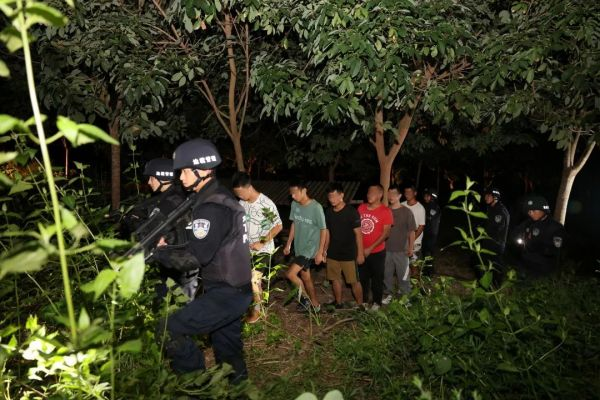
\includegraphics[width=0.35\textwidth]{1}
}
\subfloat[2022特大非法越境案件]{
	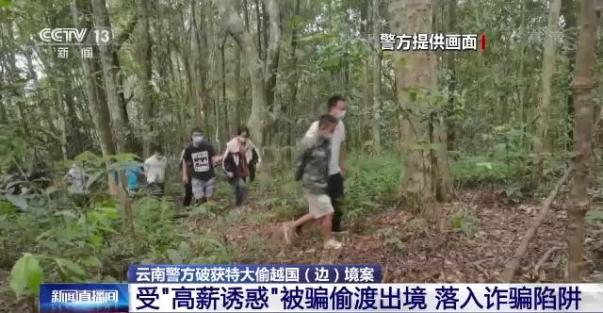
\includegraphics[width=0.45\textwidth]{2}
}\\
% \subfloat[演员王星被拐前形象]{
% 	
\includegraphics[width=0.3\textwidth]{1-1}
% }
% \subfloat[演员王星被拐后照片]{
% 	
\includegraphics[width=0.3\textwidth]{1-2}
% }
\captionsetup{justification=centering} %图题居中
\caption{近年云南非法越境案件}
\label{fig:case-}
\end{figure}

打击非法越境是一个超大场景下全天候的目标发现任务,监控系统需要在几十到几千米的较大地理空间范围内对目标进行监控,还需要实现7x24小时全气候条件下的监控覆盖。边境公安针对该问题正积极探索并应用前沿监控技术,以替代传统的警员巡逻模式,旨在克服传统手段中巡逻覆盖范围有限、反应速度滞后以及难以实现全天候、全方位监控等固有缺陷,同时有效应对日益隐蔽化和智能化的非法过境手段。然而,现有监控设备在技术层面仍存在显著不足,特别是缺乏高科技手段(如智能识别系统、多光谱成像、无人机协同巡查等)的深度集成,导致对非法过境行为的精准判断与打击能力未能达到预期效果。因此,目前超大场景安防监控有如下现实需求:
\begin{itemize}[left=15pt,label={\textasteriskcentered}]
\item 由于边境地区地形复杂多样,涵盖高山、丛林、河流等多种地貌,且环境动态变化频繁,导致监控设备在应对超大场景内物体随天气、时间变化导致的光线、能见度以及物体形态变化时,监控算法适应性和稳定性明显下降或实效。这不仅限制了设备对环境的感知能力,还影响了监控系统的稳定性和可靠性,进而制约了边境监控的效能。因此,边境安防迫切需要开发能够适应复杂地形和动态环境变化的监控设备,以提升边境监控系统的整体性能和可靠性;
\item 现有监控设备在超大场景内的潜在目标主动预测与定位能力存在显著不足。当前监控系统主要依赖被动式监控模式,缺乏基于数据分析的主动预测机制,难以对非法越境目标的出现位置、行为轨迹及潜在风险进行实时预测与精准预判。这一技术短板导致边境安防工作长期处于被动监控模式,难以在非法活动发生前采取有效干预措施,从而降低了整体防控效能。因此,边境安防迫切需要研发具备主动预测与定位能力的监控系统,通过大数据分析和智能化技术,实现对潜在目标的实时预测和有效预判,从而提升边境安防的主动防御能力和整体防控效能;
\item 针对边境地区超大场景监控的需求,现有监控设备存在明显的局限性。一方面,监控范围狭小导致在超大场景下的监控部署与运维成本居高不下,尤其是在云南省4060公里长的边境线上,单一摄像头的监控范围受限,难以实现无缝覆盖。另一方面,现有设备主要依赖被动式监控模式,无法通过调整摄像头的俯仰角、转动角及焦距主动搜索和发现超大场景下的目标,仍需依赖人力调整。因此,亟需研发具备宽广监控范围、主动搜索能力和智能化调整功能的监控系统,以降低监控部署与运维成本,进一步提升边境地区的整体防控效能。

\end{itemize}


本项目旨在通过运用大数据分析与机器学习技术,将人工干预的被动监控模式转变为算法实时控制的主动预测与搜索模式,提升监控设备在超大场景下的自主监控能力,从而有效治理非法越境问题,保障国家主权安全,推动边疆地区经济社会发展,为国家的稳定和发展创造良好环境。


\subsection{国内外研究现状及发展动态分析}

为了实现边境安防系统前述需求,现有研究主要围绕以下三个领域展开:(1)(2)(3)

本项目旨在解决现有超大场景监控安防方面的突出问题,具体涉及(1)超大动态场景下的跨领域图像特征提取;(2)超大场景下的主动目标位置预测;(3)


不足:
1. 监控设备无法有效应对超大场景中物体形态、位置和光照等因素的变化,即使较为微小的变化也可能导致监控无法正确提取场景特征
2. 在边境线形成的超大场景中,监控设备的选址往往较为固定,不能动态的调整和监控目标出现概率大的区域
3. 无法主动在大场景下通过调整摄像设备的转角、俯仰、和焦距以自动搜索目标,非常依赖大量警力定时定点巡逻,午夜往往会形成监控盲区和漏洞

挑战:
1. 大场景下现有模型训练与迁移成本与场景数量成比例增加
2. 
3. 覆盖大场景搭建与运维成本太过巨大

内容:
1. 图片特征泛化
2. 动态图预测
3. 大场景主动搜索

科学问题:
1. 大场景图像到图的转化及其表示学习,使得模型摆脱对图像局部数据的单一依赖
2. 
3.

首先,云南边境地区地形复杂,涵盖高山、丛林、河流等多种地貌,不同的景观设的自动化监控设备不能有效获取

许多区域人迹罕至,难以实现全面覆盖的监控网络,这为非法越境活动提供了天然的隐蔽条件。

其次,边境线长达4060公里,现有的监控设施和技术手段难以满足全天候、全方位的监控需求,尤其是在偏远地区,监控盲区较多,导致非法越境活动有机可乘。

最后,边境安防资源的分配不均衡,边防力量、资金和设备的投入有限,难以应对日益复杂和隐蔽的非法越境手段。例如,部分边境区域缺乏先进的监控设备(如红外探测、无人机巡逻等),导致对非法越境活动的实时监测和快速响应能力不足。这些安防监控的不足不仅加剧了非法越境问题的复杂性,也对边境地区的安全治理提出了更高的要求。因此,加强边境安防监控技术的研发与应用,优化资源配置,构建智能化、立体化的监控体系,是解决非法越境问题的关键路径之一。
















导致云南边境非法越境问题的原因是多方面的,涉及地理、经济、社会、政治等多个维度。首先,地理因素是非法越境问题的重要诱因。云南边境地形复杂,许多区域人迹罕至,难以实施全面监控,加之边境线漫长,有限的边防力量难以覆盖所有区域,这为非法越境活动提供了可乘之机。其次,经济发展不平衡是非法越境问题的重要驱动因素。云南边境地区与邻国如缅甸、老挝的经济发展水平存在较大差距,部分邻国居民为改善生活条件,选择非法进入中国。同时,边境地区部分居民生活贫困,容易受到非法活动的诱惑,参与走私、偷渡等行为。社会与文化因素也在其中扮演了重要角色。云南边境地区居住着多个跨境民族,如傣族、景颇族等,他们与邻国居民在语言、文化、血缘上有着密切联系,这种跨境联系为非法越境提供了便利。此外,部分边境地区社会治理能力薄弱,基层管理存在漏洞,难以有效遏制非法活动。

政治与法律因素同样不可忽视。邻国如缅甸长期存在政治动荡和武装冲突,导致大量难民和非法移民涌入云南边境,进一步加剧了非法越境问题的复杂性。跨境犯罪活动往往涉及多国,法律管辖和执法合作存在困难,难以形成有效的打击合力。技术与资源的限制也是边境管理面临的重要挑战。边境地区监控设施和技术手段相对落后,难以实现全天候、全方位的监控,而边防力量、资金和设备的分配也难以满足实际需求,导致部分边境区域管理薄弱。

云南边境非法越境问题不仅是一个区域性问题,更是涉及国家安全、社会稳定、经济发展和生态保护的综合性挑战。深入研究这一问题具有重要的理论和现实意义。从理论角度来看,通过多学科交叉研究,可以构建边境非法越境问题的理论框架,丰富边境治理和跨境管理的理论研究。从现实角度来看,研究成果可为政府制定边境管理政策、优化资源配置、提升治理能力提供科学依据,有助于维护边境安全、促进区域经济发展和社会稳定。因此,针对云南边境非法越境问题的研究具有重要的科学价值和社会意义。













免责声明:敬请大家仔细对比本模版与官方word转pdf后的差别,自行确定是否采用。
取消正文tex这一行注释即可对比:\verb|%\renewcommand{\input}[1]|\\
\verb|{\vspace{\baselineskip}}|。
个人认为,2025年系统仍然上传PDF,只要人眼无法分辨与官方区别,就可以。

\subsection{编译方法}
\begin{enumerate}
	\item 编译:XeLaTex->bibtex->XeLaTeX->XeLaTeX
	\item 排错:多看编译错误,多查询错误解决方法;编译警告,只要不影响PDF,就不用管。本模版多人使用,可以认为不存在编译错误。
	\item 自定义格式:多阅读一下nsfc.sty,可以解决你绝大部分问题。超过nsfc.sty范围的,建议不要想办法定制,事倍功半。
\end{enumerate}


\subsection{编辑方法}
%%%%%%%%
%\newpage
\vspace{-5pt}

\begin{figure}[h!]
	\centering %图片居中
	\includegraphics[width=6cm]{figures/xiugai.png}
	\captionsetup{justification=centering} %图题居中
	\caption{项目文件夹结构}
\end{figure}
只需要修改上图中蓝色选中区域文件即可。其他剩余文件,可以直接采用模版替换,编译就是最新版。

\subsubsection{章节}\label{subsubsec:t}
\verb|\label{subsubsect:t}|
引用章节\verb|\ref{subsubsec:t}|,生成为:\ref{subsubsec:t}。这个样式可能不是你想要的,那种情况下,就手敲吧!申请书不像论文,这种情况应该没几个。

\subsubsection{字体}
中文\textbf{粗体};\textbf{bold} font;
中文\textit{斜体};\textit{italic} font;

克制使用以下标注(不用更好),防止专家眼花缭乱。\textul{添加下划线};\textull{添加双下划线};\textuw{添加下弯线};\textud{添加下点线}。

全文改宋体,可以修改nsfc.sty的MS部分字体。

可选的就是\verb|\zhkai,\enkai,\zhsong,\ensong|。

\subsubsection{文献}
普通引用\cite{test};上标引用\citess{test};多篇文章\citess{test,test2,test3}。

有注音的英文:\cite{test}。

参考期刊\cite{test};
参考图书\cite{test2};
参考会议\cite{test5};
参考链接\cite{test4};
参考文件\cite{test6}。

对于中文参考文献,bib条目中需要有language = {zh},参见\cite{test2}。
\subsubsection{列表}
无序列表\footnote{值得注意的是,不需要一定要用列表环境,用加粗、换行、缩进同样能达到效果。
	因为咱们的初衷,还是LaTeX在排版文献和公式上有优势,发挥这一个优势就行了,其他部分不需要强行套用。文本本身还是最重要、需要大家投入精力的部分。}的例子:
\begin{itemize}[left= 50pt]
	\item[-] 第一条,第一条的内容可能很长长长长长长长长长长长长长长长长长长长长;
	\item[-] 第二条。
\end{itemize}

有序列表的例子:
\begin{enumerate}[left= 50pt]
	\item 第一条,第一条的内容可能很长长长长长长长长长长长长长长长长长长长长;
	\item 第二条。
\end{enumerate}

两个带圈文字的实现方法:
\textcircled{\raisebox{-0.8pt}{1}}
\textcircled{\textbf{\small 1}}

注意,由于列表的缩进,不同使用者可能偏向并不一样。本模版用的enumitem包,阅读他的文档进行个性化,其文档在:https://www.ctan.org/pkg/enumitem


\subsubsection{公式}

公式如下:
\begin{equation}
	E=mc^2
\end{equation}
公式的上下间距参见nsfc.sty中公式上下间距部分。

\subsubsection{图}
图片的例子:
\begin{figure}[h!]
\centering %图片居中
\includegraphics[width=2cm]{figures/IMG.JPG}
\captionsetup{justification=centering} %图题居中
\caption{这是图题}
\end{figure}

图题和表头若想取消加粗,去掉nsfc.sty中caption部分的\verb|\bfseries|即可。


\subsubsection{表}
在表格内的第一行设置\verb|\zhkai\ensong\selectfont|,来选择字体。

其中\verb|\zhkai\zhsong\enkai\ensong|可以根据需要选择。
\begin{table}[htbp]
	\zhkai\ensong\selectfont%设置表格字体
	\centering  % 显示位置为中间
	\caption{表格}  % 表格标题
	\label{table1}  % 用于索引表格的标签
	%字母的个数对应列数,|代表分割线
	% l代表左对齐,c代表居中,r代表右对齐
	\begin{tabular}{|c|c|c|c|}  
		\hline  % 表格的横线
		& & & \\[-6pt]  %可以避免文字偏上来调整文字与上边界的距离
		第一列&第二列&第三列&第四列 \\  % 表格中的内容,用&分开,\\表示下一行
		\hline
		& & & \\[-6pt]  %可以避免文字偏上 
		0.1&0.2&0.3&0.4 \\
		\hline
	\end{tabular}
\end{table}

\subsection{某页最后一段行距可能很窄?}
如果没有这个问题,就不用管这个事情。

行间距变化一般是在“多行蓝色模版”部分前后。因为蓝色模版文字在section里写的,latex把蓝色部分当作一个整体,可能硬要挤到这一页,而不是换新一页,导致会挤前一页的行间距,导致前一页行距异常。
针对这种情况,模版已经使用
\begin{lstlisting}[language=tex, basicstyle=\ttfamily\small, keywordstyle=\color{blue}, commentstyle=\color{gray}]
	%自动段落的行间距微调
	\usepackage{setspace}
	\setstretch{1.6} % 22 bp / 14 pt = 1.571
\end{lstlisting}
降低了这种情况发生的可能。
如果还有,就只好添加\verb|\newpage|把它newpage到后一页上,就行了。也可以考虑分段缓解,需要写的时候注意页面的分段和字数。

\begin{REF}
\subsection*{参考文献}
\vspace{-50pt}
\bibliographystyle{template/latex/gbt7714-nsfc}
\bibliography{sections/a6参考文献}%参考文献
\end{REF}

\newpage%自己判断是否需要
\end{MS}

\section{\textbf{项目的研究内容、研究目标,以及拟解决的关键科学问题}(此部分为重点阐述内容)\textbf{;}}

\begin{MS}
	\subsection{研究内容}

\subsubsection*{\bfseries (1)xx}


\begin{figure}[h!]
	\centering %图片居中
	\includegraphics[width=2cm]{figures/IMG.JPG}
	\captionsetup{justification=centering} %图题居中
	\caption{这是图题}
\end{figure}

\begin{table}[htbp]
	\zhkai\ensong\selectfont%设置表格字体
	\centering  % 显示位置为中间
	\caption{表格}  % 表格标题
	\label{table1}  % 用于索引表格的标签
	%字母的个数对应列数,|代表分割线
	% l代表左对齐,c代表居中,r代表右对齐
	\begin{tabular}{|c|c|c|c|}  
		\hline  % 表格的横线
		& & & \\[-6pt]  %可以避免文字偏上来调整文字与上边界的距离
		第一列&第二列&第三列&第四列 \\  % 表格中的内容,用&分开,\\表示下一行
		\hline
		& & & \\[-6pt]  %可以避免文字偏上 
		0.1&0.2&0.3&0.4 \\
		\hline
	\end{tabular}
\end{table}

\subsection{研究目标}

\subsection{拟解决的关键科学问题}

\end{MS}

\section{\textbf{拟采取的研究方案及可行性分析}(包括研究方法、技术路线、实验手段、关键技术等说明);}

\begin{MS}
	%公式的上下间距
\setlength{\abovedisplayskip}{0pt}
\setlength{\belowdisplayskip}{0pt}





\subsection{研究方案与技术路线}

\begin{figure}[h!]
\centering 

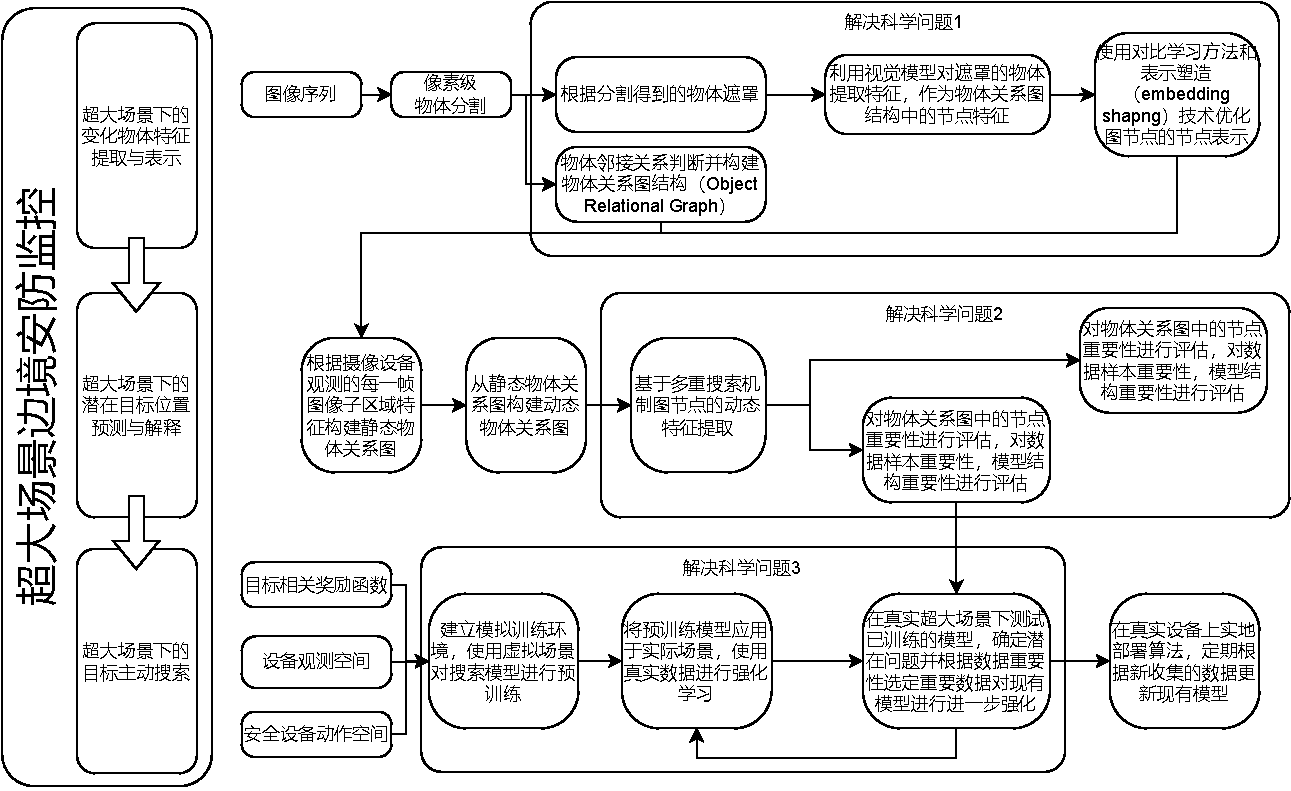
\includegraphics[width=0.9\textwidth]{figures/framework.pdf}

\captionsetup{justification=centering}
\caption{总体框架图}
\label{fig:framework}
\end{figure}

% 在\textbf{图表示学习}阶段,我们首先收集并标注包含鸟类和其他物体(如水草、藻类等)的图片。使用目标检测算法(如 Faster R-CNN 或 YOLO)提取图片中的物体及其位置信息,将每个物体表示为图中的一个节点,物体之间的关系(如距离和角度)表示为边。接着,通过图神经网络(如 \textit{GCN})对图进行卷积操作,聚合节点及其邻居的信息,更新节点的特征表示。最后,将所有节点的特征汇聚为一个全局向量 \( H_{\text{global}} \),这个向量捕捉了图中所有节点和边的信息,为后续的方向和距离预测提供了基础。

\begin{figure}[h!]
\centering %图片居中
\subfloat[数据处理&特征提取]{
	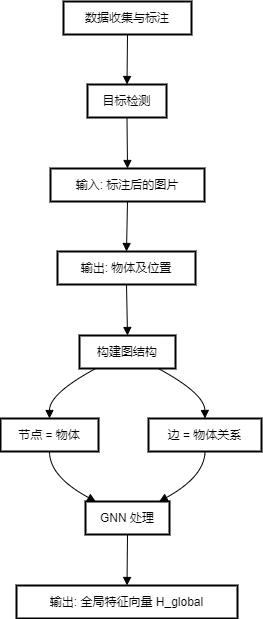
\includegraphics[width=0.35\textwidth]{figures/数据处理.drawio.png}
}
\end{figure}

\paragraph{}
说明:
数据收集与标注:获取带标注的鸟类图片数据。
目标检测:提取图片中的物体(如鸟类、背景元素)及其位置。
构建图结构:将物体作为节点,物体间关系(如空间距离)作为边。
GNN 处理:通过图神经网络生成全局特征向量。
% 
在\textbf{方向和距离回归}阶段,我们使用一个简单的神经网络(如全连接网络)作为回归模型,输入为图表示学习得到的全局向量 \( H_{\text{global}} \)。模型包含两个输出层:一个用于预测鸟类的方向(上、下、左、右),另一个用于预测鸟类与画面中心的距离。通过结合方向损失(交叉熵损失)和距离损失(均方误差损失),模型在训练阶段学习从全局向量到鸟类方位的映射关系。在监控阶段,即使当前画面中没有鸟,模型也能根据输入的全局向量实时预测鸟类可能出现的方向和距离,并指导监控摄像头转动到对应的方向,以提高监控效率。

\begin{figure}[h!]
\centering %图片居中
\subfloat[方向和距离回归]{
	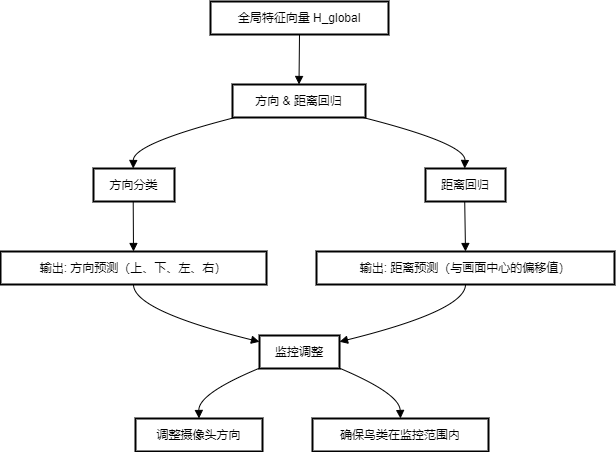
\includegraphics[width=0.9\textwidth]{figures/方向和距离回归.drawio.png}
}
\end{figure}

\paragraph{}
说明:
方向和距离回归:基于全局特征预测鸟类的位置方向(分类)和距离(回归)。
监控调整:根据预测结果实时调整摄像头,保持鸟类在画面中心。

\subsection{研究方法}

\subsection{可行性分析} 




\end{MS}

\section{\textbf{本项目的特色与创新之处;}}

\begin{MS}
	\textbf{(1)特色}

\begin{itemize}[left=30pt,itemsep=1em,label={\textasteriskcentered}]

\item \textbf{紧迫性:} 随着全球安全形势的日益复杂,跨境犯罪、恐怖主义等活动对国家边防安全构成了严重威胁。研发先进的边防主动预测与搜索技术,可以有效提升边防部门对这些威胁的感知和应对能力,保障国家的安全和稳定。因此,加快边防主动预测与搜索技术的研发,对于提升国家边防安全水平具有重要意义。
\item \textbf{推广应用前景:} 边防主动预测与搜索技术在未来的推广应用前景非常广阔。
首先,边防主动预测与搜索技术能够实现对边境地区的实时监控和智能预警,有效提高边防安全和防御能力,可以应用于边境管控、缉私缉毒、人员管控等多个场景;其次,通过技术共享,主动预测与搜索技术还能促进我国边境全域范围内边境安全的共同提升。

\end{itemize}

\textbf{(2)创新}

\begin{itemize}[left=30pt,itemsep=1em,label={\textasteriskcentered}]

\item 针对超大场景下变化物体特征有效提取问题,提出基于图结构的特征抽象方法,提升了复杂地形地貌下的特征提取完整性。
\item 针对关键动态图结构与网络模块获取与解释问题,提出动态图迭代查询与解释方法,提升稀疏观测下的特征有效利用率和图节点重要性可解释性。
\item 针对多条件优化的强化学习算法收敛慢的问题,提出多条件强化学习快速训练方法,提升强化学习代理网络的训练效率和推理质量。

\end{itemize}
\end{MS}

\section{\textbf{年度研究计划及预期研究结果}\kg{0.2em}(包括拟组织的重要学术交流活动、国际合作与交流计划等)。}

\begin{MS}
	\subsection{年度研究计划}
本课题将围绕超大场景安防监控背景下,变化目标主动预测与搜索过程中的几个关键技术开展研究,开展过程中,将广泛参与国内外高水平学术会议,研究成果拟投稿 ICML、ICLR、NeurIPS 等国际顶级会议和 IEEE TPAMI、Pattern Recognition、计算机学报、软件学报、自动化学报等国内外权威期刊。研究计划在 4 年内完成,具体如下:

\textbf{2026年1月1日-2026年12月31日}

\begin{enumerate}[left=30pt,label=(\arabic*),itemsep=1em]
\item 专家咨询与资料收集:咨询边防监控领域的专家,了解监控场景的特点和需求。收集相关资料,包括超大场景监控的图像数据、监控设备的性能参数等;
\item 场景模拟与数据准备:拍摄实验室周围场景的视频,模拟超大场景边防监控环境。对拍摄的视频进行处理,提取图像序列,构建数据集;
\item 图像分割与特征图构建:研究现有的图像分割方法,如基于CNN,BERT和Mamba的分割算法。利用这些方法对模拟场景和真实边防图像序列进行分割,构建变化物体的特征图结构;
\item GNN特征提取与初步分析:将构建的特征图结构输入图神经网络(GNN),进行特征提取。分析提取的特征,为后续的目标位置预测提供基础;
\item 年度小结,撰写不少于 2 篇高质量论文并投稿,申请国家发明专利 1 件以上。
\end{enumerate}

\textbf{2027年1月1日-2027年12月31日}

\begin{enumerate}[left=30pt,label=(\arabic*),itemsep=1em]
\item 动态图构建与分析:基于第一年构建的特征图结构序列,构建动态图。分析动态图的结构和特性,为后续的条件概率分布学习提供基础;
\item 条件概率分布学习:使用GNN学习动态图上的条件概率分布。通过训练模型,估计目标出现的可能位置;
\item 可信度评估:研究GNN的可解释性方法,如基于注意力机制的解释方法。利用这些方法评估图结构和网络模块对预测结果的可信度;
\item 结果分析与优化:分析预测结果和可信度评估结果,优化模型和算法;
\item 年度小结,撰写不少于 2 篇高质量论文并投稿,申请国家发明专利 1 件以上,参加国际或国内会议 1 次。
\end{enumerate}

\textbf{2028年1月1日-2028年12月31日}

\begin{enumerate}[left=30pt,label=(\arabic*),itemsep=1em]
\item 强化学习算法设计:基于场景中目标出现位置的可信预测,设计强化学习算法,然后定义奖励函数和状态转移函数,为摄像头的控制提供决策依据;
\item 摄像头控制策略:使用强化学习算法训练摄像头控制策略,并通过与环境的交互,学习最优的摄像头控制策略,实现高效稳定的目标搜索;
\item 实验验证与优化:在模拟和真实的边防监控环境中进行实验验证,并根据实验结果,优化强化学习算法和摄像头控制策略;
\item 结果分析与总结:分析实验结果,总结基于强化学习的摄像头控制方法的优点和不足。
\item 年度小结,撰写不少于 2 篇高质量论文并投稿,申请国家发明专利 1 件以上,参加国际或国内会议 1 次。
\end{enumerate}

\textbf{2029年1月1日-2029年12月31日}

\begin{enumerate}[left=30pt,label=(\arabic*),itemsep=1em]
\item 软硬件平台设计:根据前三年的研究成果,设计软硬件平台,包括数据采集模块、特征提取模块、目标预测模块、摄像头控制模块等。
\item 系统集成与测试:将各个模块集成到一个完整的系统中,并在实验室环境中进行初步测试,检查系统的功能和性能。
\item 实地测试与调优:将系统部署到边境进行实地测试。根据实际的边防监控场景,对系统进行调优,提高系统的稳定性和准确性。
\item 结果总结与推广:总结实地测试的结果,撰写项目总结报告,同时将研究成果进行推广,为边防监控提供新的技术手段。
\end{enumerate}










\subsection{预期研究结果}
本项目预期取得如下研究结果:

\begin{itemize}[left=15pt,,itemsep=1em,label={\textasteriskcentered}]
\item 建立超大场景下动态目标主动预测与搜索的关键技术体系;
\item 构建基于图结构抽象的变化场景及目标特征提取方法、基于稀疏观测的动态图可信预测方法以及多约束条件下强化学习模型快速训练模式;
\item 开发面向边境区域超大场景主动目标预测与搜索软硬件平台 1 套;
\item 发表 CCF 推荐 A、B 类中英文期刊及会议论文 4-6 篇;
\item 申请国家发明专利 2-3 项;
\item 撰写课题研究报告 1 份;
\item 培养研究生 4-5 名。
\end{itemize}
\end{MS}

\chapter{\textbf{研究基础与工作条件}}
\section{\textbf{研究基础}\kg{0.2em}(与本项目相关的研究工作积累和已取得的研究工作成绩);}

\begin{MS}
	

这里可能需要列出自己的相关文章。由于文章和依据部分的文献的格式并不一定一致,建议使用下边方法:
\begin{lstlisting}[language=tex, basicstyle=\ttfamily\tiny, keywordstyle=\color{blue}, commentstyle=\color{gray}]
	\begin{thebibliography}{1}
		\bibitem{test}
		\bibauthor{\textbf{C\"aldognetto T\@, Tenti P}}\@. 
		\bibtitle{Microgrids Operation Based on Master–Slave Cooperative Control}
		\bibmark{[J]}\@.
		\bibjournal{IEEE Journal of Emerging and Selected Topics in Power Electronics}\@,
		\bibvolume{2}\bibnumber{(4)}\thinspace{}\textnormal{:}
		\bibpages{1081\thinspace{}\textnormal{--}\thinspace{}1088}\@,
		\bibyear{2014}\@.
		\url{doi: 10.1109/JESTPE.2014.2345052}\@.
	\end{thebibliography}
\end{lstlisting}
效果如下。这个东西从哪里来的呢?从编译产生的\verb|.bbl|文件中拷贝过来放进来,就可以了。
\vspace{-50pt}
\begin{thebibliography}{1}
	\providecommand{\bibauthor}[1]{#1}
	\providecommand{\bibeditor}[1]{#1}
	\providecommand{\bibtranslator}[1]{#1}
	\providecommand{\bibtitle}[1]{#1}
	\providecommand{\bibbooktitle}[1]{#1}
	\providecommand{\bibjournal}[1]{#1}
	\providecommand{\bibmark}[1]{#1}
	\providecommand{\bibcountry}[1]{#1}
	\providecommand{\bibpatentid}[1]{#1}
	\providecommand{\bibedition}[1]{#1}
	\providecommand{\biborganization}[1]{#1}
	\providecommand{\bibaddress}[1]{#1}
	\providecommand{\bibpublisher}[1]{#1}
	\providecommand{\bibinstitution}[1]{#1}
	\providecommand{\bibschool}[1]{#1}
	\providecommand{\bibvolume}[1]{#1}
	\providecommand{\bibnumber}[1]{#1}
	\providecommand{\bibversion}[1]{#1}
	\providecommand{\bibpages}[1]{#1}
	\providecommand{\bibmodifydate}[1]{#1}
	\providecommand{\bibcitedate}[1]{#1}
	\providecommand{\bibyear}[1]{#1}
	\providecommand{\bibdate}[1]{#1}
	\providecommand{\biburl}[1]{\newline\url{#1}}
	\bibitem{test}
	\bibauthor{\textbf{C\"aldognetto T\@, Tenti P}}\@. \bibtitle{Microgrids Operation Based
		on Master–Slave Cooperative Control}\bibmark{[J/OL]}\@. \bibjournal{IEEE
		Journal of Emerging and Selected Topics in Power Electronics}\@,
	\bibvolume{2}\bibnumber{(4)}\thinspace{}\textnormal{:
	}\bibpages{1081\thinspace{}\textnormal{--}\thinspace{}1088}\@,
	\bibyear{2014}\@. \url{doi: 10.1109/JESTPE.2014.2345052}\@.
\end{thebibliography}
\end{MS}

\section{\textbf{工作条件}\kg{0.2em}(包括已具备的实验条件,\kg{0.2em}尚缺少的实验条件和拟解决的途径,包括利用国家实验室、全国重点实验室和部门重点实验室等研究基地的计划与落实情况);}

\begin{MS}
	xx

\end{MS}

\section{\textbf{正在承担的与本项目相关的科研项目情况}\kg{0.3em}(申请人和主要参与者正在承担的与本项目相关的科研项目情况,包括国家自然科学基金的项目和国家其他科技计划项目,要注明项目的资助机构、\kg{0.1em}项目类别、\kg{0.1em}批准号、\kg{0.1em}项目名称、获资助金额、起止年月、与本项目的关系及负责的内容等);}

\begin{MS}
	xx项目
\end{MS}


\section{\textbf{完成国家自然科学基金项目情况}\kg{0.2em}(对申请人负责的前一个资助期满的科学基金项目(项目名称及批准号)完成情况、后续研究进展及与本申请项目的关系加以详细说明。另附该项目的研究工作总结摘要(限500字)和相关成果详细目录)。}

\begin{MS}
	xx项目
\end{MS}

\chapter{\textbf{其他需要说明的情况}}
\section{申请人同年申请不同类型的国家自然科学基金项目情况\kg{0.2em}(列明同年申请的其他项目的项目类型、项目名称信息,并说明与本项目之间的区别与联系;已收到自然科学基金委不予受理或不予资助决定的,无需列出)。}

\begin{MS}
	xx项目


\end{MS}

\section{具有高级专业技术职务\kg{0.3em}(职称)\kg{0.3em}的申请人或者主要参与者是否存在同年申\kg{0.1em}请\kg{0.1em}或者\kg{0.1em}参与申请国家自然科学基金项目的单位不一致的情况;如存在上述情况,列明所涉及人员的姓名,申请或参与申请的其他项目的项目类型、项目名称、单位名称、上述人员在该项目中是申请人还是参与者,并说明单位不一致原因。}

\begin{MS}
	无


\end{MS}

\section{具有高级专业技术职务\kg{0.3em}(职称)\kg{0.3em}的申请人或者主要参与者是否存在与正在承担的国家自然科学基金项目的单位不一致的情况;如存在上述情况,列明所涉及人员的姓名,正在承担项目的批准号、项目类型、项目名称、单位名称、起止年月,并说明单位不一致原因。}

\begin{MS}
	无


\end{MS}

\section{同年以不同专业技术职务\kg{0.3em}(职称)\kg{0.3em}申请或参与申请科学基金项目的情况(应详细说明原因)。}

\begin{MS}
	无


\end{MS}

\section{其他。}

\begin{MS}
	无


\end{MS}

在\textbf{图表示学习}阶段,我们首先收集并标注包含鸟类和其他物体(如水草、藻类等)的图片。使用目标检测算法(如 Faster R-CNN 或 YOLO)提取图片中的物体及其位置信息,将每个物体表示为图中的一个节点,物体之间的关系(如距离和角度)表示为边。接着,通过图神经网络(如 \textit{GCN})对图进行卷积操作,聚合节点及其邻居的信息,更新节点的特征表示。最后,将所有节点的特征汇聚为一个全局向量 \( H_{\text{global}} \),这个向量捕捉了图中所有节点和边的信息,为后续的方向和距离预测提供了基础。

\begin{figure}[h!]
\centering %图片居中
\subfloat[数据处理&特征提取]{
	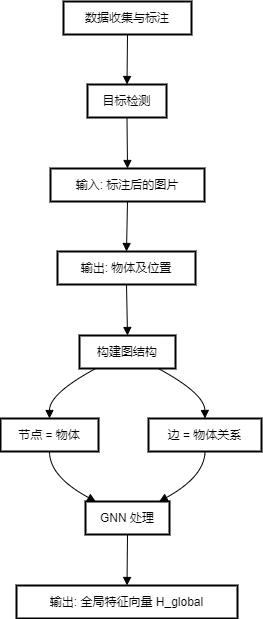
\includegraphics[width=0.35\textwidth]{figures/数据处理.drawio.png}
}
\end{figure}

\paragraph{}
说明:
数据收集与标注:获取带标注的鸟类图片数据。
目标检测:提取图片中的物体(如鸟类、背景元素)及其位置。
构建图结构:将物体作为节点,物体间关系(如空间距离)作为边。
GNN 处理:通过图神经网络生成全局特征向量。

在\textbf{方向和距离回归}阶段,我们使用一个简单的神经网络(如全连接网络)作为回归模型,输入为图表示学习得到的全局向量 \( H_{\text{global}} \)。模型包含两个输出层:一个用于预测鸟类的方向(上、下、左、右),另一个用于预测鸟类与画面中心的距离。通过结合方向损失(交叉熵损失)和距离损失(均方误差损失),模型在训练阶段学习从全局向量到鸟类方位的映射关系。在监控阶段,即使当前画面中没有鸟,模型也能根据输入的全局向量实时预测鸟类可能出现的方向和距离,并指导监控摄像头转动到对应的方向,以提高监控效率。

\begin{figure}[h!]
\centering %图片居中
\subfloat[方向和距离回归]{
	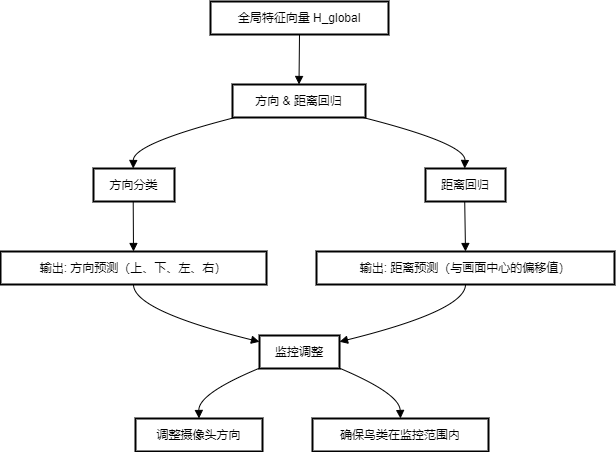
\includegraphics[width=0.9\textwidth]{figures/方向和距离回归.drawio.png}
}
\end{figure}

\paragraph{}
说明:
方向和距离回归:基于全局特征预测鸟类的位置方向(分类)和距离(回归)。
监控调整:根据预测结果实时调整摄像头,保持鸟类在画面中心。

\end{document}
